\documentclass[12pt]{article}
\usepackage{geometry}                % See geometry.pdf to learn the layout options. There are lots.
\geometry{letterpaper}                   % ... or a4paper or a5paper or ... 
%\geometry{landscape}                % Activate for for rotated page geometry
\usepackage{booktabs}
\usepackage{multirow}
\usepackage{graphicx}
\usepackage{amssymb}

\usepackage{fontspec,xltxtra,xunicode}
\defaultfontfeatures{Mapping=tex-text}
\setromanfont[Mapping=tex-text]{Hoefler Text}
\setsansfont[Scale=MatchLowercase,Mapping=tex-text]{Gill Sans}
\setmonofont[Scale=MatchLowercase]{Andale Mono}

\title{Homework 2}
\author{Yepei Zhang 912465089}
%\date{}                                           % Activate to display a given date or no date

\begin{document}
\maketitle

1.\\

(a). $R(A,B,C,D,E)$\quad $AB\rightarrow E, B\rightarrow C, CE\rightarrow A, AE\rightarrow D$\\
$A^{+} = \{A\}$\quad $B^{+}=\{B,C\}$\quad$C^{+} = \{C\}$\quad $D^{+} = \{D\}$\quad $E^{+} = \{E\}$\quad $AB^{+} = \{A,B,C,D,E\}$\\
$AC^{+} = \{A,C\}$\quad $AD^{+} = \{A,D\}$\quad $AE^{+} = \{A,D,E\}$\quad $BC^{+} = \{BC\}$\\
$BD^{+} = \{B,C,D\}$\quad $BE^{+} = \{A,B,C,D,E\}$\quad $CD^{+} = \{C,D\}$\quad $CE^{+} = \{A,C,D,E\}$\\
$DE^{+} = \{D,E\}$\quad $ABC^{+} = \{A,B,C,D,E\}$\quad $ABD^{+} = \{A,B,C,D,E\}$\\
$ABE^{+} = \{A,B,C,D,E\}$\quad $ACD^{+} = \{A,C,D\}$\quad $ACE^{+} = \{A,C,D,E\}$\\
$ADE^{+} = \{A,D,E\}$\quad $BCD^{+} = \{B,C,D\}$\quad $BCE^{+} = \{A,B,C,D,E\}$\\
$BDE^{+} = \{A,B,C,D,E\}$\quad $CDE^{+} = \{A,C,D,E\}$\quad $ABCD^{+} = \{A,B,C,D,E\}$\quad $BCDE^{+} = \{A,B,C,D,E\}$\\

keys: $\{A,B\}\quad \{B,E\}$\\

(b). $AB^{+} = \{A,B,C\}$, by using FDs except $AB\rightarrow E$, this closure doesn't include E. Thus, $AB\rightarrow E$ is not implied by other three FDs.\\
Similarly, we can get $B^{+} = \{B\}$ doesn't include C, $CE^{+} = \{C,E\}$ doesn't include A, $AE^{+} = \{A,E\}$ doesn't include D. Thus, the set of the FDs is a minimal basis.\\

(c). FDs: \quad $AB\rightarrow E,\ B\rightarrow C,\ CE\rightarrow A,\ AE\rightarrow D,\ AB\rightarrow C,\ AB\rightarrow D,\ BE\rightarrow A,\ BE\rightarrow C,\ BE\rightarrow  D,\ BD\rightarrow C,\ CE\rightarrow D,\ ABC\rightarrow D,\ ABC\rightarrow E,\ ABD\rightarrow C,\ ABD\rightarrow E,\ ABE\rightarrow C,\ ABE\rightarrow D,\ ACE\rightarrow D,\ BCE\rightarrow A,\ BCE\rightarrow D,\ BDE\rightarrow A,\ BDE\rightarrow C,\ CDE\rightarrow A,\ ABCD\rightarrow E,\ BCDE\rightarrow A$\\
BCNF violations: $B\rightarrow C,\ CE\rightarrow A,\ AE\rightarrow D,\ BD\rightarrow C,\ CE\rightarrow D,\ ACE\rightarrow D, CDE\rightarrow A$\\

(d). Start with the BCNF violation $B\rightarrow C$, we get $R_{1}(B,C)$, with key $\{B\}$, FD $B\rightarrow C$ which is a minimal basis.\\
$R_{2}(A,B,D,E)$, key $\{A,B\}$, FDs $AB\rightarrow E,\ AE\rightarrow D$, the second FD violates BCNF, continue decomposing. \\
$R_{21}(A,E,D)$, key $\{A,E\}$, FD $AE\rightarrow D$ which is a minimal basis and doesn't violate BCNF.\\
$R_{22}(A,B,E)$, key $\{A,B\}$, FD $AB\rightarrow E$ which is a minimal basis and doesn't violate BCNF.\\ 
Thus, the decomposed relations: $\{B,C\},\ \{A,E,B\},\ \{A,E,D\}$\\

(e). 3NF violations: $B\rightarrow C,\ AE\rightarrow D,\ BD\rightarrow C,\ CE\rightarrow D, ACE\rightarrow D$\\

(f). We can see from (b) that the given set FDs is a minimal basis. Thus, the 3NF decomposition is $S_{1}(A,B,E),\ S_{2}(B,C),\ S_{3}(A,C,E),\ S_{4}(A,D,E)$. Here, $S_{1}(A,B,E)$ includes the key $\{A,B\}$, thus, there is no need adding another relation.\\

(g). From (c), we have known all FDs and BCNF violations. According to FD promotion, we know some of the 4NF MVD violations: $B\rightarrow\rightarrow C,\ CE\rightarrow\rightarrow A,\ AE\rightarrow\rightarrow D,\ BD\rightarrow\rightarrow C,\ CE\rightarrow\rightarrow D,\ ACE\rightarrow\rightarrow D,\ CDE\rightarrow\rightarrow A$\\
Then, according to complementation rule, we get other 4NF MVD violations. $B\rightarrow\rightarrow ADE,\ CE\rightarrow\rightarrow BD,\ AE\rightarrow\rightarrow  BC,\ BD\rightarrow\rightarrow AE,\ CE\rightarrow\rightarrow AB,\ ACE\rightarrow\rightarrow B,\ CDE\rightarrow\rightarrow B$\\

(h). Start with the violation $B\rightarrow\rightarrow C$, we get $R_{1}(B,C)$. key: $\{B\}$, FD: $B\rightarrow C$, MVD: $B\rightarrow\rightarrow C$, there is no 4NF violation.\\
$R_{2}(A,B,D,E)$. key $\{A,B\}$, FDs: $AB\rightarrow E,\ AE\rightarrow D$, MVDs: $AB\rightarrow\rightarrow E,\ AE\rightarrow\rightarrow D,\ etc.$, one of the violation is $AE\rightarrow\rightarrow D$.\\
$R_{21}(A,D,E)$. key $\{A,E\}$, FD: $AE\rightarrow D$, MVD:$AE\rightarrow\rightarrow D$\\
We can use chase test to check if $A\rightarrow\rightarrow D$ holds.\\

\begin{tabular}{|c|c|c|}
\hline
A & D & E  \\
\hline
$a$ & $d$ & $e_{1}$  \\
\hline
$a$ & $d_{1}$ & $e$  \\
\hline
\end{tabular}\\

However, there is no useful FD we can apply further to make it agree on D column. Thus, $A\rightarrow\rightarrow D$ doesn't hold. Similarly, $A\rightarrow\rightarrow E$ doesn't hold. 



$R_{22}(A,B,E)$. key $\{A,B\}$, FD: $AB\rightarrow E$, MVD:$AB\rightarrow\rightarrow E$\\
If we use chase test to check if $A\rightarrow\rightarrow E$ or $B\rightarrow\rightarrow E$ hold, similar situation as $R_{21}$ shows that there is no more FD making any change to make it agree on some column. 
Thus, the 4NF decomposition: $\{B,C\},\ \{A,D,E\},\ \{A,B,E\}$. FDs and MVDs are listed above.\\

(i). $S(A,B,C)$\qquad $A^{+} = \{A\},\ B^{+} = \{B, C\},\ C^{+} = \{C\},\ AB^{+} = \{A, B, C\},\ BC^{+} = \{B, C\},\ AC^{+} = \{A, C\}$
 clearly the key is $\{A,B\}$, $B\rightarrow C$ holds \\
Thus, the nontrivial FDs: $B\rightarrow C,\ AB\rightarrow C$\qquad nontrivial MVDs: $B\rightarrow\rightarrow C,\ B\rightarrow\rightarrow A$\\
Apply chase test to check it there is other nontrivial MVDs.\\
If we want to check if $A\rightarrow\rightarrow C$ holds:\\

\begin{tabular}{|c|c|c|}
\hline
A & B & C  \\
\hline
$a$ & $b_{1}$ & $c$  \\
\hline
$a$ & $b$ & $c_{1}$  \\
\hline
\end{tabular}\\

We can see that given FDs and MVDs cannot be applied anymore, because it agrees only on A column. However, there is no FDs or MVDs with A on the left hand side alone. Similarly, we cannot find $A\rightarrow\rightarrow B$ hold.\\
Then, check if $C\rightarrow\rightarrow A$ holds:\\

\begin{tabular}{|c|c|c|}
\hline
A & B & C  \\
\hline
$a$ & $b_{1}$ & $c$  \\
\hline
$a_{2}$ & $b$ & $c$  \\
\hline
\end{tabular}\\

We can see that given FDs and MVDs cannot be applied anymore, because it agrees only on C column. However, there is no FDs or MVDs with C on the left hand side alone. Similarly, we cannot find $C\rightarrow\rightarrow B$ hold.\\

In brief: the nontrivial FDs: $B\rightarrow C,\ AB\rightarrow C$\qquad nontrivial MVDs: $B\rightarrow\rightarrow C,\ B\rightarrow\rightarrow A$\\



2.\\
(a). Start with the tableau:\\

\begin{tabular}{|c|c|c|c|c|c|}
\hline
C & T & H & R & S & G \\
\hline
$c_{1}$ & $t_{1}$ & $h$ & $r_{1}$ & $s$ & $g_{1}$ \\
\hline
$c_{2}$ & $t_{2}$ & $h$ & $r_{2}$ & $s$ & $g_{2}$\\
\hline
\end{tabular}\\

Apply $HR\rightarrow R$, then $r_{2}=r_{1}$\\

\begin{tabular}{|c|c|c|c|c|c|}
\hline
C & T & H & R & S & G \\
\hline
$c_{1}$ & $t_{1}$ & $h$ & $r_{1}$ & $s$ & $g_{1}$ \\
\hline
$c_{2}$ & $t_{2}$ & $h$ & $r_{1}$ & $s$ & $g_{2}$\\
\hline
\end{tabular}\\

Apply $HR\rightarrow C$, then $c_{2}=c_{1}$\\

\begin{tabular}{|c|c|c|c|c|c|}
\hline
C & T & H & R & S & G \\
\hline
$c_{1}$ & $t_{1}$ & $h$ & $r_{1}$ & $s$ & $g_{1}$ \\
\hline
$c_{1}$ & $t_{2}$ & $h$ & $r_{1}$ & $s$ & $g_{2}$\\
\hline
\end{tabular}\\

Apply $CS\rightarrow G$, then $g_{2}=g_{1}$\\

\begin{tabular}{|c|c|c|c|c|c|}
\hline
C & T & H & R & S & G \\
\hline
$c_{1}$ & $t_{1}$ & $h$ & $r_{1}$ & $s$ & $g_{1}$ \\
\hline
$c_{1}$ & $t_{2}$ & $h$ & $r_{1}$ & $s$ & $g_{1}$\\
\hline
\end{tabular}\\

Thus two tuples now agree in the G column. $HG\rightarrow G$ holds.\\

(b). Start with the tableau:\\

\begin{tabular}{|c|c|c|c|c|c|}
\hline
C & T & H & R & S & G \\
\hline
$c_{1}$ & $t$ & $h$ & $r$ & $s_{1}$ & $g_{1}$ \\
\hline
$c_{2}$ & $t$ & $h$ & $r$ & $s_{2}$ & $g_{2}$\\
\hline
\end{tabular}\\

Apply $HR\rightarrow C$, then $c_{2}=c_{1}$\\

\begin{tabular}{|c|c|c|c|c|c|}
\hline
C & T & H & R & S & G \\
\hline
$c_{1}$ & $t$ & $h$ & $r$ & $s_{1}$ & $g_{1}$ \\
\hline
$c_{1}$ & $t$ & $h$ & $r$ & $s_{2}$ & $g_{2}$\\
\hline
\end{tabular}\\

When we apply $C\rightarrow T,\ HT\rightarrow R,\ HS\rightarrow R$, there is nothing changed. We cannot get two tuples agree on S. So $THR\rightarrow S$ doesn't hold.\\

(c).Start with the tableau:\\

\begin{tabular}{|c|c|c|c|c|c|}
\hline
C & T & H & R & S & G \\
\hline
$c$ & $t$ & $h$ & $r_{1}$ & $s_{1}$ & $g_{1}$ \\
\hline
$c$ & $t_{2}$ & $h$ & $r$ & $s_{2}$ & $g$\\
\hline
$c$ & $t_{3}$ & $h_{3}$ & $r$ & $s$ & $g_{3}$\\
\hline
\end{tabular}\\

The first two rows agree on C and H, apply $C\rightarrow T$, so they agree on T. $t_{2}=t$\\

\begin{tabular}{|c|c|c|c|c|c|}
\hline
C & T & H & R & S & G \\
\hline
$c$ & $t$ & $h$ & $r_{1}$ & $s_{1}$ & $g_{1}$ \\
\hline
$c$ & $t$ & $h$ & $r$ & $s_{2}$ & $g$\\
\hline
$c$ & $t_{3}$ & $h_{3}$ & $r$ & $s$ & $g_{3}$\\
\hline
\end{tabular}\\

Then the first two rows agree on T,H,C, apply $HT\rightarrow R$, then $r_{1}=r$\\

\begin{tabular}{|c|c|c|c|c|c|}
\hline
C & T & H & R & S & G \\
\hline
$c$ & $t$ & $h$ & $r$ & $s_{1}$ & $g_{1}$ \\
\hline
$c$ & $t$ & $h$ & $r$ & $s_{2}$ & $g$\\
\hline
$c$ & $t_{3}$ & $h_{3}$ & $r$ & $s$ & $g_{3}$\\
\hline
\end{tabular}\\

Then, the first two rows agree on C,T,H,R. No more change can be made because of the given FDs. There is no row that is fully unsubscripted. Thus, this decomposition doesn't have a lossless join.\\

(d). Firstly, check whether the set of FDs is a minimal basis.\\
$HR^{+} = {H,R}$ doesn't include C after applying FDs except $HR\rightarrow C$. Similarly, $HT^{+} = {H,T},\ HS^{+} = {H,S},\ CS^{+} = {C, S, T},\ C^{+} = {C},\ $ Thus, the given set of FDs is a minimal basis.\\
Then, we can get relations: $S_{1}(C,T),\ S_{2}(H,R,C),\ S_{3}(H,R,T), S_{4}(H,S,R), S_{5}(C,S,G)$. We note that the key is $\{H,S\}$ which is included into $S_{4}(H,S,R)$. Thus, we are done.\\

(e).\\
Decompose R into BCNF.\\
Begin from $C\rightarrow T$, we get $R_{1}(C, T)$ key: $\{C\}$ FD: $C\rightarrow D$\\
$R_{2}(C, H, R, S, G)$, key: $\{H, S\}$, FDs: $HR\rightarrow C$(violation), $HS\rightarrow R,\ HS\rightarrow G,\ CS\rightarrow G$(violation).\\
$R_{21}(H, R, C)$, key: $\{H, R\}$, FDs: $HR\rightarrow C$\\
$R_{22}(H, R, S, G)$, key: $\{H, S, G\}$, FD: $HS\rightarrow R$ (violation)\\
$R_{221}(H, S, R)$, key: $\{H,S\}$, FD: $HS\rightarrow R$\\
$R_{222}(H, S, G)$, key: $\{H, S, G\}$ no FD\\
Thus, BCNF decomposition is $R_{1}(C, T),\ R_{21}(H, R, C),\ R_{221}(H, S, R),\ R_{222}(H, S, G)$, keys and FDs are listed above.\\
Compare with 3NF decomposition, $\{H, R, T\}, \{C, S, G\}$ are in 3NF but not in BCNF\\


(f). Decompose R into 4NF.\\
Start with $C\rightarrow\rightarrow T$, we get $R_{1}(C, T)$, MVD: $C\rightarrow\rightarrow D$\\
$R_{2}(C, H, R, S, G)$, key: $\{H, S\}$, FDs: $HR\rightarrow\rightarrow C$(violation), $HS\rightarrow\rightarrow R,\ HS\rightarrow\rightarrow G,\ CS\rightarrow\rightarrow G$(violation).\\
$R_{21}(H, R, C)$, key: $\{H, R\}$, MVD: $HR\rightarrow\rightarrow C$\\
$R_{22}(H, R, S, G)$, key: $\{H, S, G\}$, MVDs: $HS\rightarrow\rightarrow R$ (violation), $HS\rightarrow\rightarrow G$(violation)\\
$R_{221}(H, S, R)$, key: $\{H,S\}$, MVD: $HS\rightarrow\rightarrow R$\\
$R_{222}(H, S, G)$, key: $\{H, S, G\}$\\
Thus, 4NF decomposition is $R_{1}(C, T),\ R_{21}(H, R, C),\ R_{221}(H, S, R),\ R_{222}(H, S, G)$, keys and MVDs are listed above.\\
Compare with 3NF decomposition, $\{H, R, T\}, \{C, S, G\}$ are in 3NF but not in 4NF\\



3.\\
Assume they are not getting multiple PhDs. To avoid the situation that some people have the same name, I set the key $\{name, dissertation\ title, year\ of\ graduate\}$. Academics can be students and instructors. One student have one instructor as dissertation chair, but one instructor can chair many students. That's why the relationship of "chair" is "one to many". Two instructors can be the dissertation committee members for many students. That's why the relationship of "are committee members of" is "two to many". In addition, one can have many progenies and progenitors. Thus, the relationship of "academic progeny" is "many to many". In this model, the one academic cannot play different roles at the same time, which one cannot chair himself or chair and become committee member of same person. Thus, it is a reasonable model. \\
\begin{figure}[htbp]
   \centering
   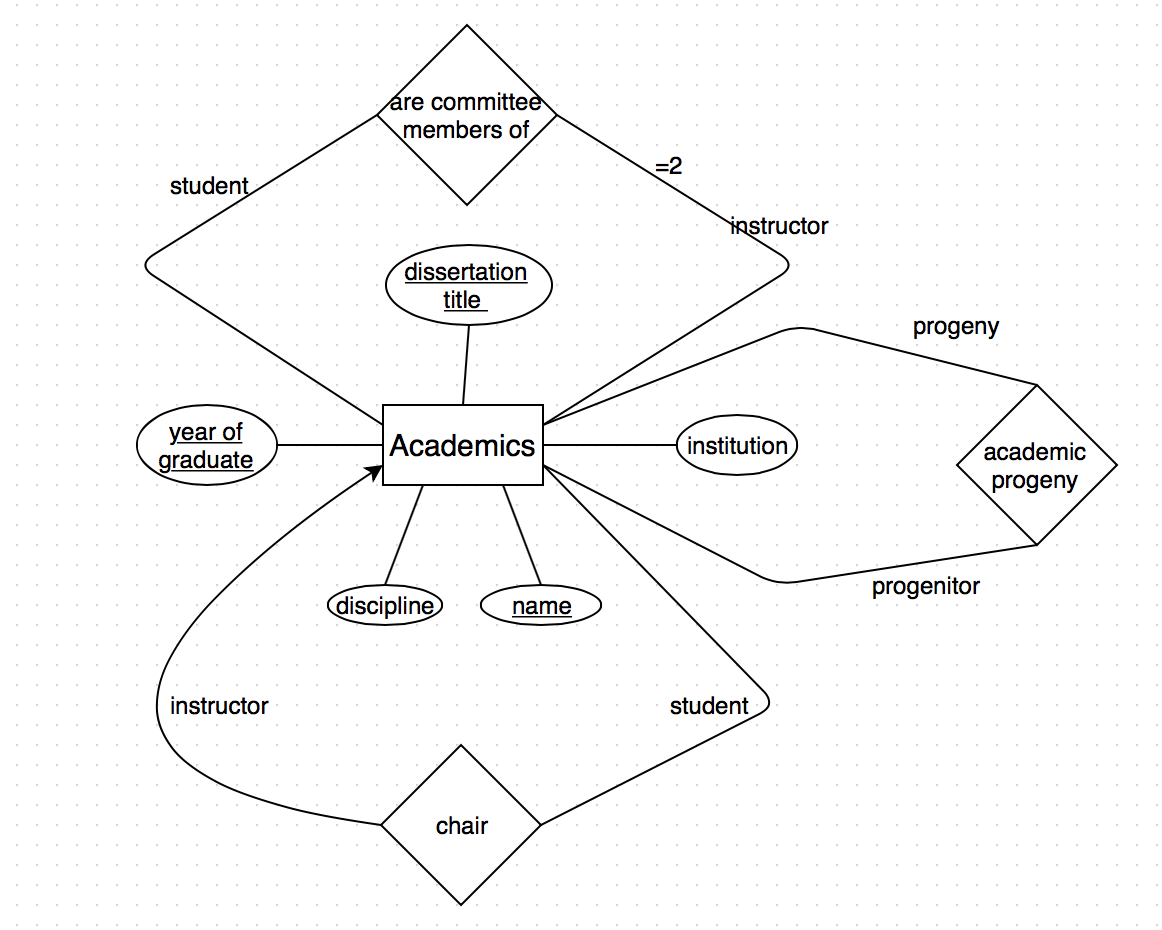
\includegraphics[width=0.8\textwidth]{diagram.png} 
\end{figure}
























\end{document}  